\documentclass[UTF8]{ctexart}
\usepackage{subfigure}
\usepackage{caption}
\usepackage{amsmath,bm}
\usepackage{amssymb}
\usepackage{pifont}
\usepackage{geometry}
\usepackage{graphicx}
\usepackage{gensymb}
\usepackage{wrapfig}
\usepackage{titlesec}
\usepackage{float}
\usepackage{diagbox}
\usepackage{fancyhdr}
\usepackage{color}
\usepackage{bm}
\usepackage{siunitx}
\usepackage{ulem}
\usepackage{CJKulem}
\pagestyle{plain}
\geometry{a4paper,scale=0.8}
\CTEXsetup[format+={\raggedright}]{section} 
\title{固物2017期末}
\author{Deschain}
\titlespacing*{\section}
{0pt}{0pt}{0pt}
\titlespacing*{\subsection}
{0pt}{0pt}{0pt}
\titlespacing*{\paragraph}
{0pt}{0pt}{0pt}
\titlespacing*{\subparagraph}
{0pt}{0pt}{0pt}
\titleformat*{\section}{\normalsize}
\begin{document}
\maketitle
\section*{1.}
(1)\ding{172}玻色子\ding{173}$\frac{1}{e^{\frac{\hbar\omega}{k_BT}}-1}$\\
(2)\ding{172}体心立方\ding{173}$\frac{2\pi}{\lVert2\vec{\beta_1}+3\vec{\beta_2}+\vec{\beta_3}\rVert}$\\
(3)\ding{172}$2:1$\ding{173}$2V_0$\\
(4)\ding{172}声学波\ding{173}升高\\
(5)\ding{172}间接\ding{173}$\hbar \vec{k}-\hbar \vec{q}$\\
(6)\ding{172}电子的轨道磁矩\ding{173}电子的自旋磁矩\ding{174}感生磁矩\ding{175}铁磁性\ding{176}亚铁磁性\ding{177}反铁磁性\\
(7)\ding{172}抗磁性\\
(8)\ding{172}$3nN$\ding{173}$3N$\ding{174}$3(n-1)N$\\
(9)\ding{172}OA上存在\ding{173}不存在\\
(10)\ding{172}高\ding{173}N\ding{174}P\\
(11)\ding{172}$[-\frac{\pi}{2a},\frac{\pi}{2a}]$\ding{173}$\sqrt{17}:1$\\
(12)\ding{172}独立\ding{173}统一\\
(13)\ding{172}$0.804$\\
(14)\ding{172}正\ding{173}下降\\
(15)\ding{172}自由电子\ding{173}$\lambda<\frac{h}{E_g}$\\
(16)\ding{172}V\ding{173}导带\\
\section*{2.}
(1)
\begin{figure}[H]                                         
    \centering                                                
    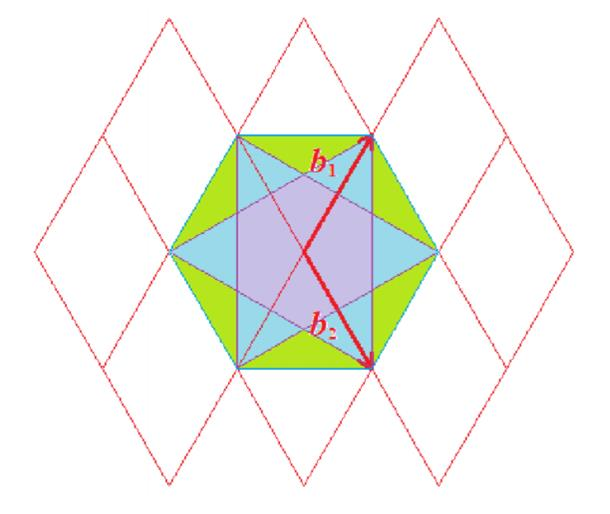
\includegraphics[width=4cm,height=4cm]{ans-2-1.jpg}        
    \caption*{}                                                                                  
\end{figure}
(2)
\begin{equation*}
    \begin{aligned}
        & k_F=\sqrt{2\pi n}=\sqrt{\frac{4\pi}{3\sqrt3 a^2}}\\
    \end{aligned}
\end{equation*}
(3)
\begin{equation*}
    \begin{aligned}
        & r=\frac{2\pi}{3a}\\
    \end{aligned}
\end{equation*}
(4)
\begin{equation*}
    \begin{aligned}
        & \sqrt{N}k_F=r, N=\frac{\pi}{\sqrt3}\\
    \end{aligned}
\end{equation*}
\section*{3.}
(1)
\begin{equation*}
    \begin{aligned}
        & N_p=N_A+N_D=2.5\times10^{17}cm^{-3},\mu_n=450, \mu_p=190\\
        & P_p=\frac{N_A-N_D}{2}+\sqrt{(\frac{N_A-N_D}{2})^2+n_i^2}=5\times10^{16}cm^{-3}\\
        & \sigma_p=\mu_pP_pq=1.52cm/\Omega\\
        & N_n = 10^{17}cm^{-3}, \mu_n=900, \mu_p=330\\
        & \sigma_n=\mu_nn_Nq=14.4cm/\Omega\\
    \end{aligned}
\end{equation*}
(2)
\begin{equation*}
    \begin{aligned}
        &E_{F_p}=E_{F_i}-k_BTln(\frac{P_p}{n_i})=E_{F_i}-0.389eV\\
        &E_{F_n}=E_{F_i}+k_BTln(\frac{N_D}{n_i})=E_{F_i}+0.407eV\\
        &V_D=0.796V\\
    \end{aligned}
\end{equation*}
\begin{figure}[H]                                         
    \centering                                                
    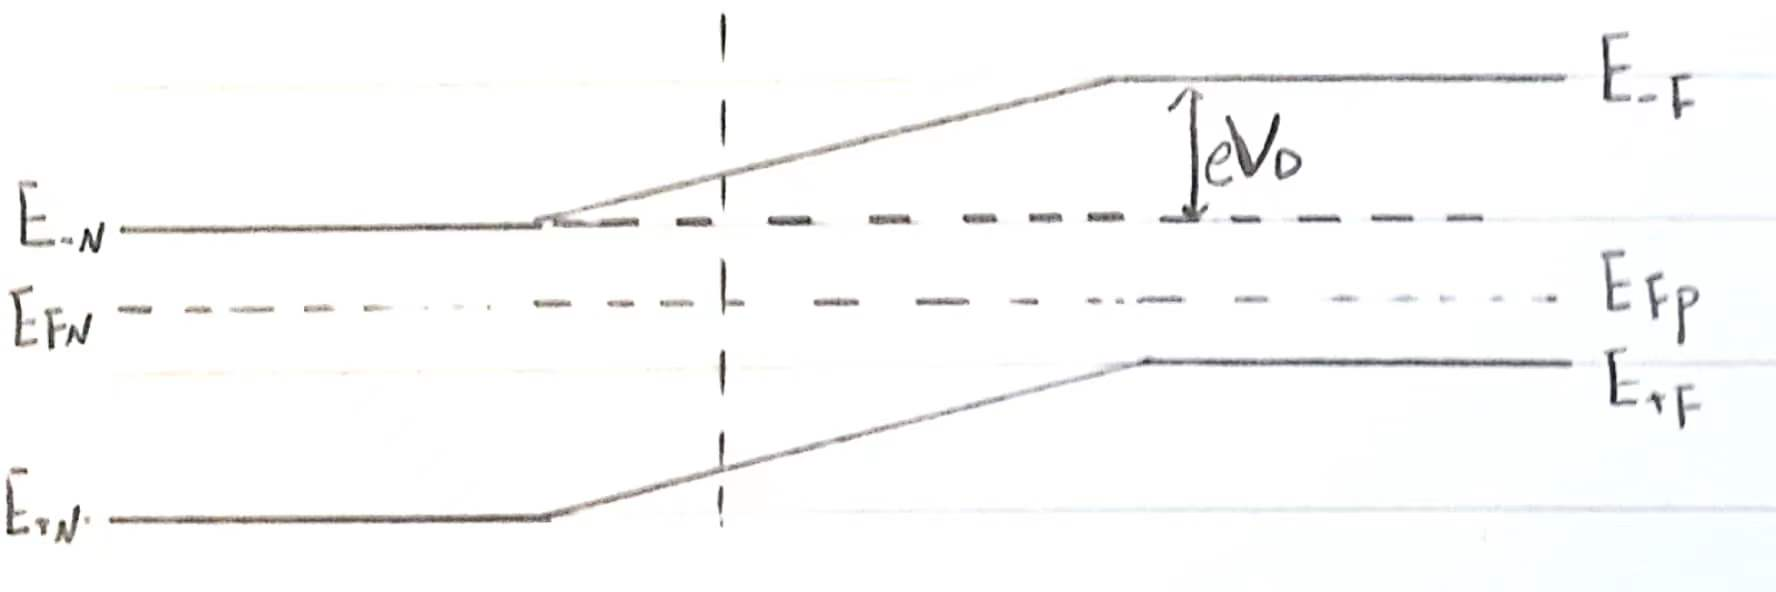
\includegraphics[width=9cm,height=3cm]{ans-3-2.jpg}        
    \caption*{}                                                                                   
\end{figure} 
(3)
\begin{equation*}
    \begin{aligned}
        & j=-q(\frac{D_n}{L_n}n_P^0+\frac{D_p}{L_p}p_N^0)=\frac{I}{S}\\
    \end{aligned}
\end{equation*}
\section*{4.}
(1)
\begin{equation*}
    \begin{aligned}
        & E(0,0,0)=A-3B, E(\frac{\pi}{a},\frac{\pi}{a},\frac{\pi}{a})=A+3B, \Delta V = 6B=3eV\\
    \end{aligned}
\end{equation*}
(2)
\begin{equation*}
    \begin{aligned}
        &v_k=\frac{1}{\hbar}\nabla E_k=\frac{aB}{\hbar}(sin(k_xa),sin(k_ya),sin(k_za))\\
    \end{aligned}
\end{equation*}
(3)
\begin{equation*}
    \begin{aligned}
        &\frac{1}{m^*}=\frac{1}{\hbar^2}\frac{\partial^2E}{\partial k^2}
        \begin{bmatrix}
            cos(k_xa)&0&0\\
            0&cos(k_ya)&0\\
            0&0&cos(k_za)\\
        \end{bmatrix}\\
        &m^*_{top} = -\frac{\hbar^2}{a^2B}(1,1,1), m^*_{bottom} = \frac{\hbar^2}{a^2B}(1,1,1)\\
    \end{aligned}
\end{equation*}
(4)
\begin{equation*}
    \begin{aligned}
        & \frac{dk}{dt}=\frac{eE}{\hbar}, t=\frac{\hbar\pi}{aeE}=6.898\times10^{-8}s\\
    \end{aligned}
\end{equation*}
(5)
\begin{equation*}
    \begin{aligned}
        &k=\frac{Eet}{\hbar}=1.518\times10^7\\
        &v_k=\frac{aB}{\hbar}(sin(k_xa),sin(k_ya),sin(k_za))=1.037\times10^3(1,1,1)m/s\\
    \end{aligned}
\end{equation*}
\section*{5.}
(1)
\begin{equation*}
    \begin{aligned}
        & E_{g_{Si}}(100)=1.101eV, E_{g_{Si}}=0.6345eV\\
    \end{aligned}
\end{equation*}
(2)
\begin{equation*}
    \begin{aligned}
        & n_{iSi}=(N_{-}N_{+})^{\frac{1}{2}}e^{-\frac{Eg_{Si}}{2k_BT}}=\frac{2}{h^3}(2\pi k_BT)^{\frac{3}{2}}
        (m_n^*m_p^*)^{\frac{3}{4}}e^{-\frac{Eg_{Si}}{2k_BT}}=9.015\times10^{11}cm^{-3}\\
        & n_{iGe}=(N_{-}N_{+})^{\frac{1}{2}}e^{-\frac{Eg_{Ge}}{2k_BT}}=\frac{2}{h^3}(2\pi k_BT)^{\frac{3}{2}}
        (m_n^*m_p^*)^{\frac{3}{4}}e^{-\frac{Eg_{Ge}}{2k_BT}}=4.660\times10^{14}cm^{-3}\\
    \end{aligned}
\end{equation*}
(3)
\begin{equation*}
    \begin{aligned}
        & \Delta E_{F_{Si}}=k_BTln(\frac{N_D}{n_i})=0.1516eV\\
        & n_{Ge}=\frac{N_D}{2}+\sqrt{(\frac{N_D}{2})^2+n_{i_{Ge}}^2}=5.187\times10^{14}cm^{-3}, 
        \Delta E_{F_{Ge}}=k_BTln(\frac{n_{Ge}}{n_i})=3.448\times10^{-3}eV\\
    \end{aligned}
\end{equation*}
(4)向Si中掺杂P的方案更好\\






\end{document}